\immediate\write18{makeindex -s nomencl.ist -o Outputs/doc.nls Outputs/doc.nlo}

\documentclass[11pt]{article}

%Langue et encodage :
 \usepackage[T1]{fontenc}
 \usepackage[utf8]{inputenc}
 \usepackage{lmodern}
 \usepackage[english]{babel} \usepackage{lmodern}


%Mise en page
\usepackage[a4paper, margin=2.5cm]{geometry}		%Papier
\usepackage{arev}									%Police
\renewcommand{\baselinestretch}{1.15} 				%Interligne
\setlength\parindent{4pt}							%Alineas
\usepackage[skip=5pt,font=footnotesize]{caption}
\usepackage{float}
\usepackage{xcolor}									%Couleurs perso
\definecolor{grisPerso}{rgb}{0.9,0.9,0.9}
%\usepackage{tabu}

%Contenu :
\usepackage{hyperref}								%Liens
\usepackage{amsmath}								%Math
\usepackage{listings}								%Code source
\lstset{
language=bash,
backgroundcolor=\color{grisPerso},
basicstyle=\footnotesize,
frame=single}
\usepackage[refpage]{nomencl}						%Nomenclature
\usepackage{xpatch}
\makenomenclature

%Dessins et schémas
\usepackage{graphicx}
\usepackage{epstopdf}
\epstopdfsetup{outdir=./}
\usepackage{subcaption}
\usepackage{tikz}
 
\newcommand{\illu}[3]{%
	\begin{figure}[H]
			  \centering
			  \includegraphics[scale=#3]{Graphics/#1}
			  \caption{#2}
			  \vspace{-5pt}
	\end{figure}}

\newcommand{\fname}[1]{\textbf{\textit{#1}}}


\newcommand{\bashCode}[1]{\colorbox{grisPerso}{\textbf{\lstinline{#1}}}}

\newcommand{\sectionWoNum}[1]{\setcounter{secnumdepth}{0}\section{#1}\setcounter{secnumdepth}{4}\setcounter{subsection}{0}}

\xpatchcmd{\thenomenclature}{%
  \section*{\nomname}% Look for `\section*... etc.
}{% Replace it by 'nothing'
}{\typeout{Success}}{\typeout{Failure}}

\xpatchcmd{\bibliography}{%
  \section*{\nomname}% Look for `\section*... etc.
}{% Replace it by 'nothing'
}{\typeout{Success}}{\typeout{Failure}}



\begin{document}

%!TEX root = ../rapport.tex

\begin{titlepage}
\newgeometry{top=2cm,bottom=2cm}

\newcommand{\HRule}{\rule{\linewidth}{0.5mm}} % Defines a new command for the horizontal lines, change thickness here

\center % Center everything on the page
 
%----------------------------------------------------------------------------------------
%   HEADING SECTIONS
%----------------------------------------------------------------------------------------


\includegraphics[scale=0.7]{Graphics/LOGO-IPSA.pdf}\\[2cm]

\Large Graduation Project \\[0.2cm] % Major heading such as course name
\large Autonomous Vehicles\\[2cm] % Minor heading such as course title

{\normalsize \today}\\[2cm]

%----------------------------------------------------------------------------------------
%   TITLE SECTION
%----------------------------------------------------------------------------------------

\HRule \\[0.5cm]
{ \Large \bfseries User Documentation}\\[0.2cm] % Title of your document
\HRule \\[2.5cm]


%----------------------------------------------------------------------------------------
%   LOGO SECTION
%----------------------------------------------------------------------------------------

 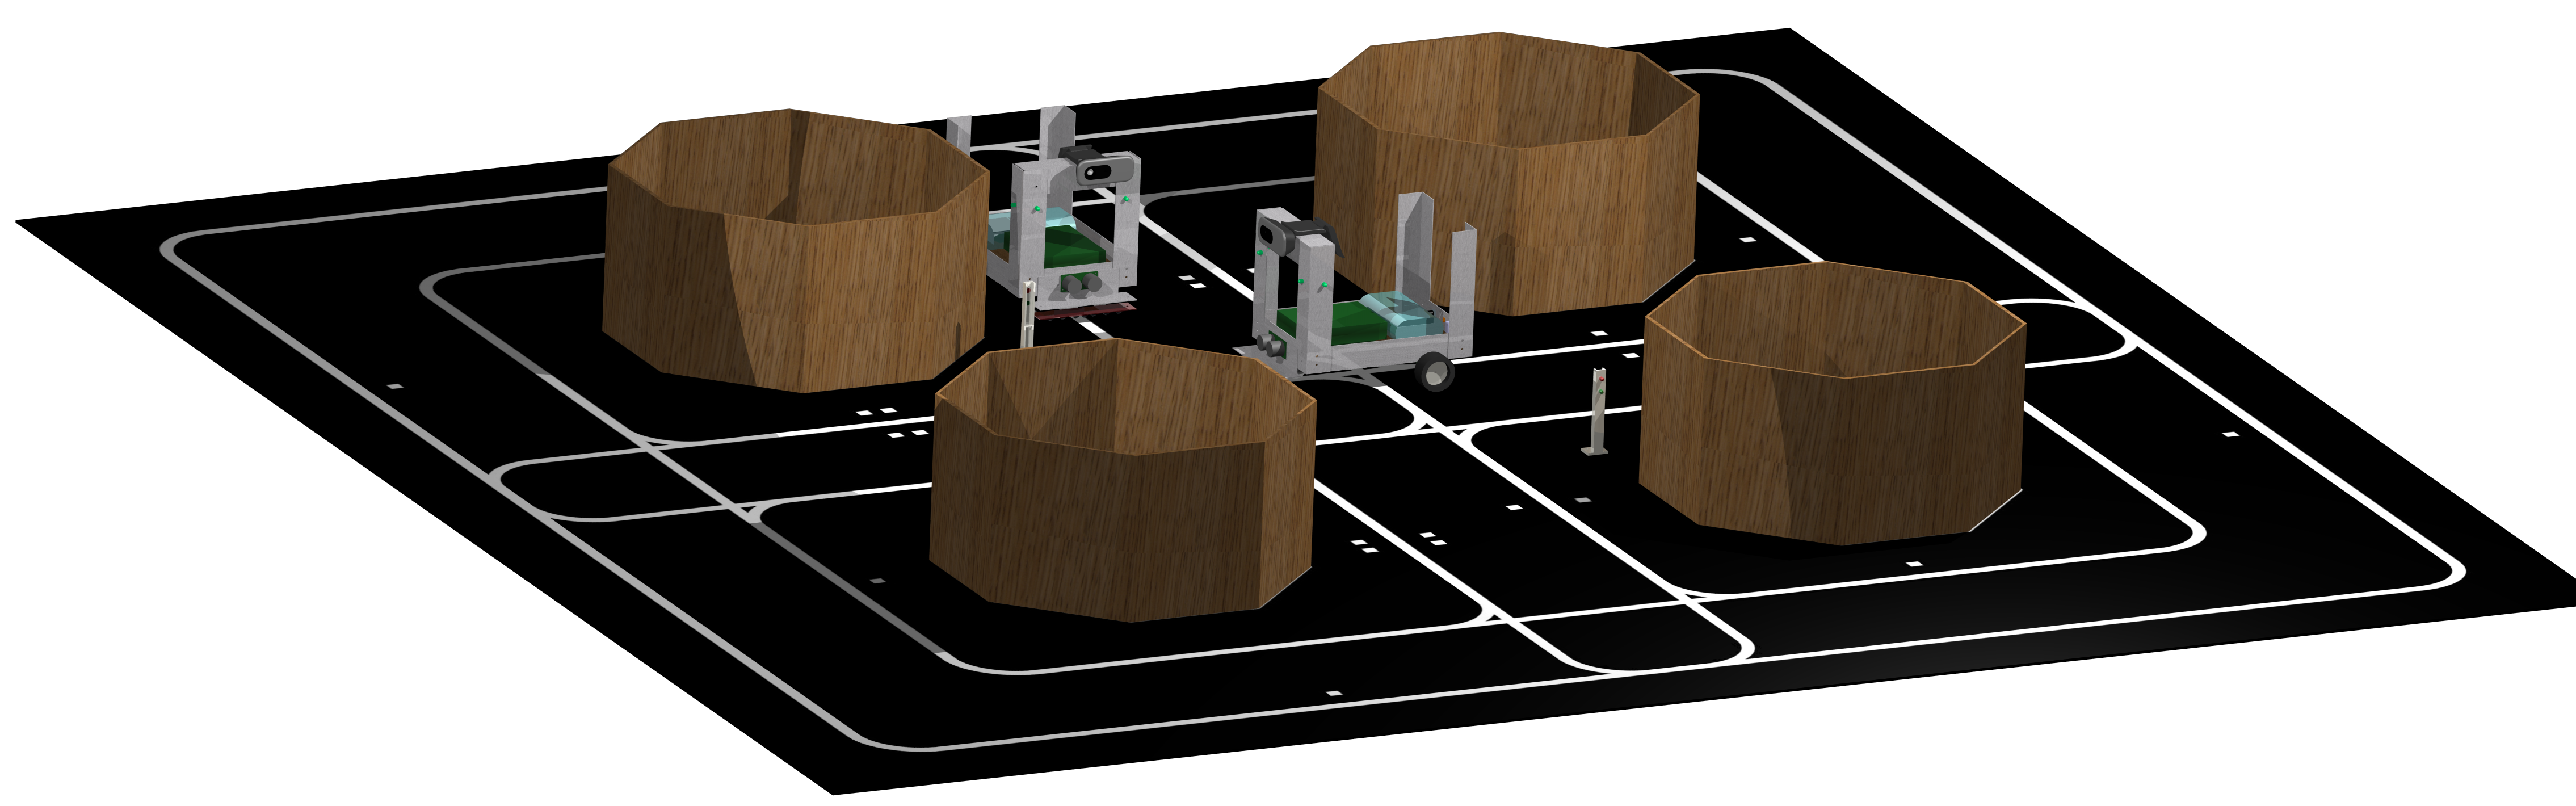
\includegraphics[scale=0.09]{Graphics/illu.png}\\[2.5cm]

%----------------------------------------------------------------------------------------
%   AUTHOR SECTION
%----------------------------------------------------------------------------------------
{\normalsize Auteurs:}\\
\small
BITON Guillaume \small(guillaume.biton@ipsa.fr)\\
MONNOT Maxime \small(maxime.monnot@ipsa.fr)\\
SON Kyeong Hwan \small(thsrudghks1@naver.com) [1cm]

 
%----------------------------------------------------------------------------------------

\vfill % Fill the rest of the page with whitespace

\restoregeometry

\end{titlepage}

\setcounter{secnumdepth}{5}
\setcounter{tocdepth}{5}

\newpage
\tableofcontents
\newpage
\pagenumbering{arabic}

\section*{Preliminary Comment}
	
 	
\newpage

\section{Introduction}

	\input{chapitres/0_introduction}

\newpage
\section{System's Objectives}

	This chapter is dedicated to explaining the project's (and therefore the system's) objectives.\\
In order to understand how the system works one has to understand what goal it is made to fulfill.\\

In this document, we will distinguish the \textbf{platform} from the \textbf{robots} and will consider them as two independant sets of systems.\\

The \textbf{platform} aims at simulating a simple set of situations a vehicle could face in an urbain environment : it has four different intersections plus a crossroad with four traffic-lights. It should provide a comfortable amount of configurations.\\
The traffic-lights are controlled from an electronic card designed to serve as a "Basys 2" FPGA card interface. They can be simply "time-programmed" or can be made a bit smarter by taking advantage of the Reed switches implemented in the "lanes" just before the traffic-lights.\\

The \textbf{robots} or \textbf{autonomous vehicles} are designed to wander along the \textbf{platform} : they should be able to stay on their lane, and move autonomously while being able to avoid all collision (yield-to-the-right, stopping on a red traffic-light...). The robot's main purpose is to serve as a test-bench. It is not made to be a perfect autonomous vehicle but should be well-made enough so that anyone willing to test autonomous-vehicle related code or algorithm can use it to perform the tests quickly and efficiently.\\
Out-of-th-box, the robots will only be able to follow a line and stop when they have to. But they should provide enough modularity so that it is easy to enhance this simple behavior. Every single aspect of the robot should be handled by a dedicated piece of software. That way, it is easy for a user to "implement" his code while taking advantage from the existing functions.

\newpage
\section{System's Description}

	\subsection{The robot}

\subsubsection{Hardware description}

\newpage
\section{RobotBasics API}

\newpage
\section{Modules Description}

\setcounter{secnumdepth}{0}
\renewcommand{\thesubsection}{\Alph{subsection}}

\newpage
\sectionWoNum{Appendices}
	%\input{chapitres/Annexes/carteCircuit}
\setcounter{secnumdepth}{0}
\newpage
\section{References}

	\subsection{Nomenclature} \label{nomenclature}
		\printnomenclature

	\newpage
	\nocite{bib11,bib1}
	\subsection{Bibliography} \label{bibliography}
		\begingroup
		\renewcommand{\section}[2]{}%
		\bibliography{includes/bibliography}{}
		\bibliographystyle{plain}
		\endgroup

	\newpage
	\subsection{Table of Figures}
		\begingroup
		\renewcommand{\section}[2]{}%
		\listoffigures
		\endgroup
		
\newpage
\section{Abstract}
	--
\end{document}